\documentclass{subfiles}
\begin{document}
\section{Time-Independent Basis for the Morse Double-Well}\label{sec:time_independent_basis}


\subsection{Exchange interaction in the basis state representation}
In our Hartree approach (Section \ref{sec:Hartree_method}) we include only the direct Coulomb interaction term between the particles, disregarding the exchange interaction as we aim to construct our system in such a way that particles are strictly localized, and thus, distinguishable. By construction this neglects any exchange effects, which - while they cannot generate entanglement - do shift single-particle levels and can in principle modify both the spectrum and the composition of our reduced basis. To test the validity of dropping exchange altogether, we compare the Hartree ground-state energy against a fully antisymmetrized treatment obtained via a truncated configuration-interaction (CI) projection \ref{sec:CI_method}. \\ 

Recall that in the Hartree product-state approach ('distinguishable particles'), the two-particle Hamiltonian
\begin{align*}
    H_{dist} = H_L \otimes \mathbb{I} + \mathbb{I} \otimes H_R + V_{LR},
\end{align*}
where $H_L$ and $H_R$ are the single-particle Hamiltonians of the left and right wells, respectively, and $V_{LR}$ is the direct Coulomb interaction between the particles. 

In the CI approach, we start from the same two-particle Hamiltonian but build a projection onto the anti-symmetric subspace spanned by all unordered pairs of single-particle states. Concretely, we form the normalized antisymmetrized two-particle combinations and  collect these as columns of the pojection matrix $P$, as shown in Section \ref{sec:CI_method}. Recall that the CI Hamiltonian is then given by
\begin{align*}
    H_{CI} = P H_{dist} P^\dagger,
\end{align*}
where $P$ is the projection operator onto the antisymmetrized subspace. This Hamiltonian inherits all one- and two-body terms from the original Hamiltonian, but now includes the exchange interaction term due to the anti-symmetrization. Diagonalization then yields the exact fermionic energy spectrum within the truncated subspace.

We carry out both calculations, Hartree and CI diagonalization as a function of inter-well separation $d$. In both solvers, we use a Sinc-DVR basis with $N=800$ gripoints and  grid length of $L=400$ a.u. This yields a gridspacing of $\Delta x = 0.5$ a.u. and a grid wide enough to encapsulate the system equally for all inter-well separations considered in the analysis. The gridspacing is chosen to be small enough to ensure convergence of the results. For CI we build the $N$ lowest single-particle orbitals and retain $\binom{N}{2}$ anti-symmetric states. We define the exchange-induced shift
\begin{align*}
    \Delta E = E_{CI} - E_{Hartree},
\end{align*}
where $E_{CI}$ is the ground-state energy obtained from the CI diagonalization and $E_{Hartree}$ is the ground-state energy obtained from the Hartree product state approach. The exchange shift $\Delta E$ quantifies the exchange interaction energy contribution, as is visualized alongside the two ground-state energies in figure \ref{fig:exchange_shift}. As the wells move farther apart, the exchange interaction energy falls off sharply, dropping below the numerical noise floor for separations $d > 10$ a.u, which is 10 $a_0$. Converted to SI units using an effective Bohr radius $a_0^* = \epsilon_r/(m^/m_e)a_o$ we are well within working ranges for quantum dots ($10-100$ nm), using a suitable semi-conductor \cite{jacak2013quantum, garcia2021semiconductor}.\textcolor{red}{TODO: We need to stay consistent with this mapping!!}
\begin{figure}[h!]
    \centering
    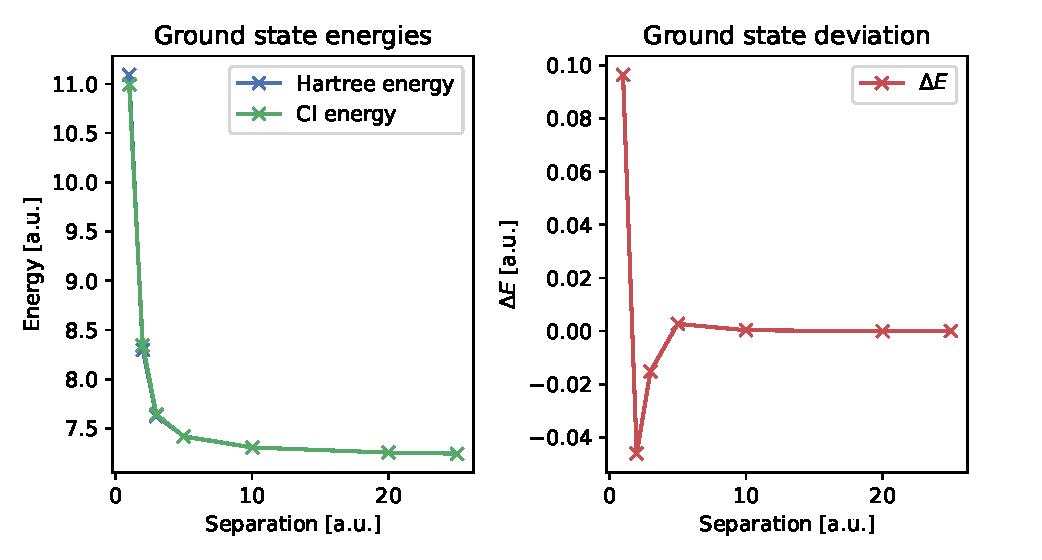
\includegraphics[width=1.0\textwidth]{figs/exchange_shift.pdf}
    \caption{Ground-state energy as a function of the inter-well separation $d$ for the Morse double-well potential. The rapid decay of the exchange term of the coulomb interaction matrix with increasing well separation indicates that this term has a negligible effect on the ground state energy, confirming our assumption of locality and the usage of product states to express the wavefunction, as the particles become distinguishable for appropriate separation. We can see that the exchange term is close to zero $eV$ for well separations larger than $d = 10$a.u. For similar separations, our product state Hartree procedure converge with the truncated CI solution. }
    \label{fig:exchange_shift}
\end{figure}
We observe that the exchange interaction has a near-zero contribution beyond moderate separations, confirming that exchange contributions are truly negligible for our system - and that the Hartree product state captures the correct low-energy physics. This vindicates our assumption that the particles are distinguishable: once the two wells are sufficiently separated, the Pauli exclusion principle has vanishing impact of both energies and wavefunctions. The parameters used for this simulations are the optimal parameters for the Morse double-well configuration $C_I$ \ref{tab:optimized_parans}, as described in section \ref{sec:optimization_procedure} and presented in Section \ref{sec:optimization_result}. 

A final caveat: because the Hartree product state is not anti-symmetric, the Hartree energy is not variational with respect to exchange (it can lie slightly below the true anti-symmetric energy in a truncated basis, as seen in figure \ref{fig:exchange_shift}). One must therefore thread carefully when interpreting the energies obtained from the Hartree product state. In our tests, however, we find no (strictly) un-physical energies - the Hartree energy is within sub meV of the CI energy for all separations considered. We therefore conclude that for all practical purposes, the product state Hartree approximation suffices and this justifies neglecting exchange in our time-evolution simulations. \textcolor{red}{TODO: More discussion needed. Should we change the plot and make an attempt to compare direct vs exchange energy instead?}

\end{document}